\documentclass[a4paper, twocolumn]{article}

\usepackage[top=2.5cm, bottom=2.5cm, left=2.5cm, right=2.5cm]{geometry}
\usepackage{graphicx}
\usepackage{amsmath}

\author{Ane Novrup Larsen, Nathasja Skov Fink Nielsen}
\title{Regression and Logistic Regression Analysis Using the Cars Dataset}
\date{October 24, 2025}

\begin{document}

\twocolumn[
    \maketitle
    
    \begin{abstract}
    This report applies two supervised learning models—multiple linear regression and logistic regression—to the \texttt{cars.csv} dataset. The linear regression model predicts a car’s acceleration time based on engine and weight features, while the logistic regression model classifies whether a car is US-made or foreign-made.
    
    Both models were trained and evaluated using standard metrics. Linear regression achieved an $R^2$ of 0.59, showing moderate predictive power. Logistic regression reached ROC AUC scores above 0.94 on both validation and test sets, indicating strong classification performance. The results demonstrate how regression techniques can be used to model both continuous and binary outcomes from structured data.
    \end{abstract}
    
    \vspace{1cm}
]

\section{Introduction\label{sec:Introduction}}
Regression models are widely used in machine learning to predict outcomes based on input features. This project applies two types of regression—linear and logistic—to a dataset of car specifications.

The goal is to demonstrate how regression techniques can model both continuous and binary outcomes. Linear regression is used to predict a car’s acceleration time, while logistic regression classifies whether a car is US-made. Both are based on features like \textit{horsepower}, \textit{displacement}, \textit{weight}, and \textit{cylinders}.

The comparison highlights both their similarities in preprocessing and their differences in evaluation and interpretation.

\subsection{Dataset Overview}
The dataset contains 398 cars with technical specifications such as \texttt{cylinders}, \texttt{displacement}, \texttt{horsepower}, \texttt{weight}, and \texttt{acceleration}, along with metadata like \texttt{model year}, \texttt{origin}, and \texttt{car name}. 
This structure allows for both regression and classification tasks using numeric and categorical features.

\section{Linear Regression Analysis}

\subsection{Methodology}
A multiple linear regression model was used to predict a car’s acceleration time (0–60 mph) from four features: \texttt{weight}, \texttt{horsepower}, \texttt{displacement}, and \texttt{cylinders}. The workflow consisted of data preparation, model training, and evaluation.

\subsubsection{Data Preparation}
The \texttt{cars.csv} dataset was cleaned by converting non-numeric \texttt{horsepower} values and removing missing rows. The inputs ($X$) included the four predictors and \texttt{acceleration} was the target ($y$). Data was split into 80\% training and 20\% testing sets.

\subsubsection{Model Training}
The model was trained using \texttt{Linear Regression} from \texttt{scikit-learn}, estimating coefficients ($\beta_i$) that define how each feature influences acceleration.

\subsubsection{Model Evaluation}
Performance was assessed using Mean Squared Error (MSE) and the coefficient of determination ($R^2$). The model achieved an $R^2$ of approximately 0.59 and an MSE of 3.04, indicating that it explains about 59\% of the variation in acceleration times.

\subsection{Results}
The fitted regression equation was expressed as:

\begin{align}
\text{acceleration} &= \beta_0 + \beta_1(\text{weight}) + \beta_2(\text{horsepower}) \nonumber \\
&\quad + \beta_3(\text{displacement}) + \beta_4(\text{cylinders})
\end{align}

The coefficients followed expected trends: \texttt{weight} had a positive coefficient, indicating that heavier cars accelerate more slowly, while \texttt{horsepower}, \texttt{displacement}, and \texttt{cylinders} had negative coefficients, showing that stronger engines reduce acceleration time. The results indicate that at least one predictor variable significantly affects the acceleration time, supporting the alternative hypothesis ($H_1$) and leading to the rejection of the null hypothesis ($H_0$).


\subsection{Conclusion}
The linear regression model effectively captured how vehicle characteristics influence acceleration. Although its predictive accuracy was moderate, it provided interpretable insights consistent with real-world automotive dynamics. Future improvements could include polynomial or regularized regression methods to better capture nonlinear relationships.


\section{Logistic Regression Analysis}

\subsection{Methodology}
A logistic regression model was used to classify cars as American-made or foreign-made based on five features: \texttt{cylinders}, \texttt{displacement}, \texttt{horsepower}, \texttt{weight}, and \texttt{acceleration}. The process included cleaning the data, scaling the features, training the model, and checking how well it performed.

\subsubsection{Data Preparation}
The \texttt{cars.csv} dataset was cleaned by removing rows with missing \texttt{horsepower} values and converting them to numeric. A new binary target column was created: cars with \texttt{origin} = 1 were labeled as 1 (US/American-made), and all others as 0 (foreign-made). The data was split into 70\% training, 15\% validation, and 15\% test sets. I scaled all features using \texttt{StandardScaler}, fitted only on the training data to prevent data leakage.

\subsubsection{Model Training}
The model was trained using \texttt{Logistic Regression} from \texttt{scikit-learn}, with no regularization (\texttt{penalty=None}) and the \texttt{lbfgs} solver. I set the tolerance to \texttt{1e-2}, which made the model stop early after 10 iterations. This configuration was selected after comparison with regularized alternatives as it has better log-loss performance.

\subsubsection{Model Evaluation}
Performance was assessed using accuracy, log-loss, and ROC AUC on the validation and test sets. The model achieved a validation ROC AUC of 0.9457 and a test ROC AUC of 0.9286. Additionally, 5-fold cross-validation on the training set gave a mean ROC AUC of 0.9435. This shows that the model performs consistently across different splits.

\subsection{Results}
The logistic regression equation looked like this:

\begin{align*}
\log\left(\frac{P(\text{US})}{1 - P(\text{US})}\right) 
&= \\
& \beta_0 + \beta_1(\text{displacement}) \\
&+ \beta_2(\text{cylinders}) + \beta_3(\text{weight}) \\
&+ \beta_4(\text{horsepower}) \\
&+ \beta_5(\text{acceleration})
\end{align*}

\begin{figure}[h]
\centering
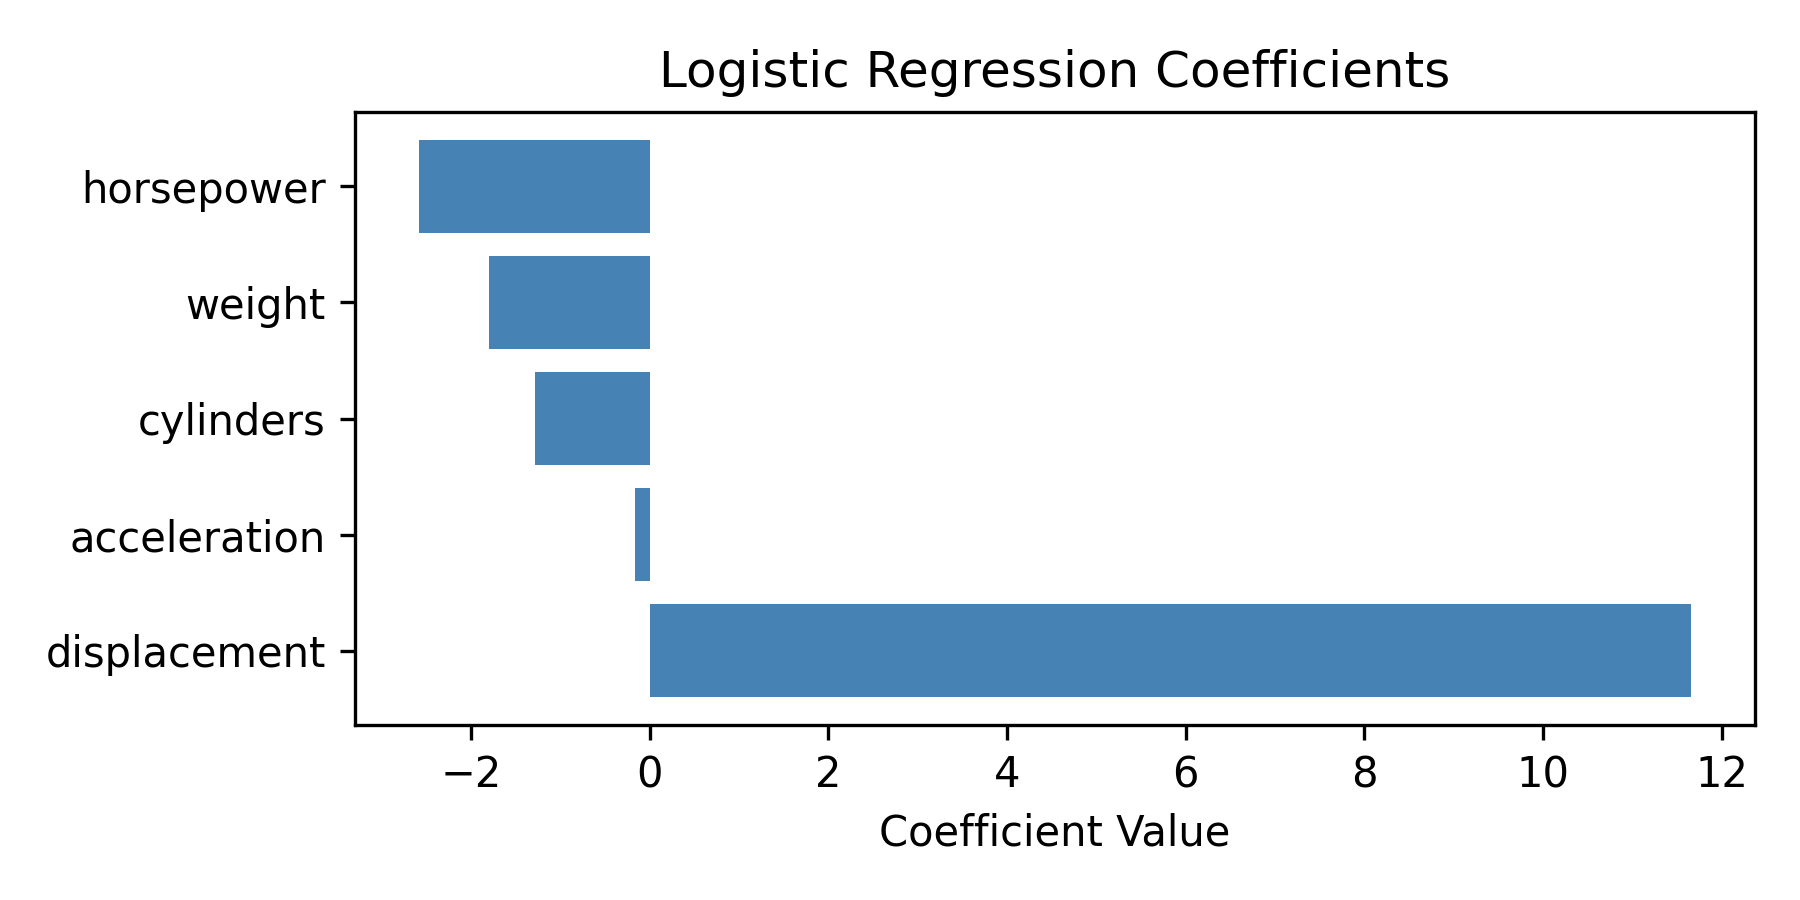
\includegraphics[width=\linewidth]{logistic_coefficients.png}
\caption{Logistic regression coefficients sorted by magnitude.}
\end{figure}

The coefficients revealed that \texttt{displacement} had the strongest positive influence on predicting American-made cars, while \texttt{horsepower}, \texttt{weight}, and \texttt{cylinders} had negative coefficients. These results support the alternative hypothesis ($H_1$), indicating that at least one feature significantly affects the classification. Therefore, the null hypothesis can be rejected.

\subsection{Conclusion}
The logistic regression model showed strong predictive performance. Its ROC AUC scores were consistent across validation and test sets, suggesting good generalization. Regularized versions were tested but gave worse log-loss, so the final setup used no penalty. Future work could explore alternative models to improve performance.

\section{Conclusion}
Both models performed well within their respective tasks. Linear regression provided interpretable insights into acceleration, while logistic regression achieved high classification accuracy. Future work could explore more complex models to improve performance further.

\end{document}